\documentclass[tikz,border=10pt]{standalone}
\usepackage{tikz}
\usetikzlibrary{arrows.meta,decorations.pathmorphing,calc}

\begin{document}
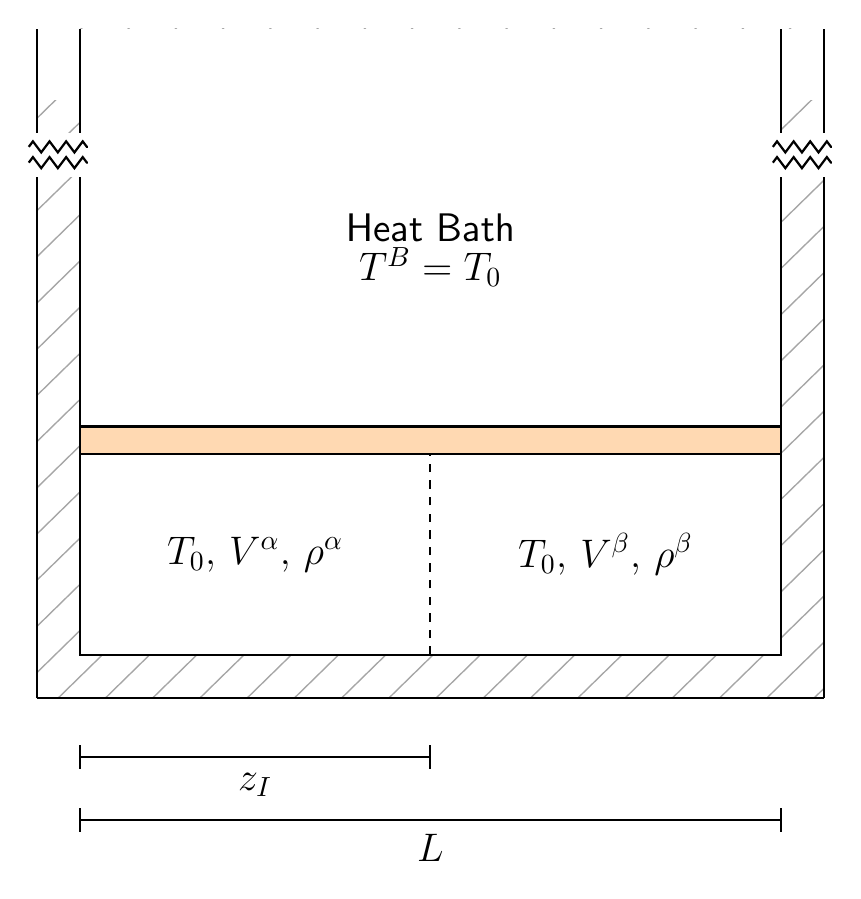
\begin{tikzpicture}
% ---------------------------------------------------------
% Dimensions (tweak freely)
% ---------------------------------------------------------
\def\TotalW{10}        % total width
\def\TotalH{8.5}       % total height (top of outer walls)
\def\WallThick{0.55}   % insulation thickness
\def\SplitY{3.1}       % top of two-phase chamber (bottom of diathermal)
\def\DiaH{0.35}        % diathermal wall thickness
\def\InnerTop{7.6}     % top of INNER cavity walls (open above this)
\def\BreakY{6.9}       % y-location of side break marks

% Derived
\pgfmathsetmacro{\InnerL}{\WallThick}
\pgfmathsetmacro{\InnerR}{\TotalW-\WallThick}
\pgfmathsetmacro{\InnerB}{\WallThick}
\pgfmathsetmacro{\MidX}{\TotalW/2}
\pgfmathsetmacro{\DiaTop}{\SplitY+\DiaH}

% Put the heat-bath label INSIDE the white bath region
\pgfmathsetmacro{\BathMidY}{(\DiaTop+\InnerTop)/2}  % middle of bath region

% ---------------------------------------------------------
% Styles
% ---------------------------------------------------------
\tikzset{
  gas style/.style={fill=white, draw=black, thick},
  dia style/.style={fill=orange!30, draw=black, thick},
  break line/.style={
    thick, decorate,
    decoration={zigzag, amplitude=2pt, segment length=6pt}
  },
  label text/.style={font=\sffamily\Large, align=center},
  math text/.style={font=\Large}
}

% =========================================================
% 1) HATCH BACKGROUND (clip to outer bounding box)
% =========================================================
\begin{scope}
  \clip (0,0) rectangle (\TotalW,\TotalH);

  \def\HatchStep{0.60} % smaller = denser hatch
  \foreach \t in {-90,...,150} {
    \draw[gray!70, line width=0.5pt]
      (-12+\t*\HatchStep, -12) -- (-12+\t*\HatchStep+45, 32);
  }
\end{scope}

% =========================================================
% 2) REMOVE TOP HATCH STRIP (OPEN TOP)
%    This is what you want: no hatched "ceiling".
% =========================================================
\fill[white] (0,\InnerTop) rectangle (\TotalW,\TotalH);

% =========================================================
% 3) MASK INTERIOR REGIONS (erase hatch where "fluid" is)
% =========================================================
% Heat bath interior region (white)
\fill[white] (\InnerL,\DiaTop) rectangle (\InnerR,\InnerTop);

% Two-phase chamber region
\filldraw[gas style] (\InnerL,\InnerB) rectangle (\InnerR,\SplitY);

% Diathermal wall (orange slab)
\filldraw[dia style] (\InnerL,\SplitY) rectangle (\InnerR,\DiaTop);

% =========================================================
% 4) DRAW CONTAINER BORDERS (outer U + inner U)
% =========================================================
% Outer U (no top edge)
\draw[thick] (0,0) -- (\TotalW,0);
\draw[thick] (0,0) -- (0,\TotalH);
\draw[thick] (\TotalW,0) -- (\TotalW,\TotalH);

% Inner U (no top edge)
\draw[thick] (\InnerL,\InnerB) -- (\InnerR,\InnerB);
\draw[thick] (\InnerL,\InnerB) -- (\InnerL,\InnerTop);
\draw[thick] (\InnerR,\InnerB) -- (\InnerR,\InnerTop);

% =========================================================
% 5) SIDE BREAK MARKS (zigzags on the insulated walls)
% =========================================================
% Left break: erase then draw zigzags, then restore wall edges
\fill[white] (-0.1, \BreakY-0.28) rectangle (\WallThick+0.1, \BreakY+0.28);
\draw[break line] (-0.1, \BreakY+0.10) -- (\WallThick+0.1, \BreakY+0.10);
\draw[break line] (-0.1, \BreakY-0.10) -- (\WallThick+0.1, \BreakY-0.10);

% Restore vertical border lines (outer + inner wall edges)
\draw[thick] (0,0) -- (0,\BreakY-0.28);
\draw[thick] (0,\BreakY+0.28) -- (0,\TotalH);
\draw[thick] (\WallThick,\InnerB) -- (\WallThick,\BreakY-0.28);
\draw[thick] (\WallThick,\BreakY+0.28) -- (\WallThick,\TotalH);

% Right break
\fill[white] (\TotalW-\WallThick-0.1, \BreakY-0.28) rectangle (\TotalW+0.1, \BreakY+0.28);
\draw[break line] (\TotalW-\WallThick-0.1, \BreakY+0.10) -- (\TotalW+0.1, \BreakY+0.10);
\draw[break line] (\TotalW-\WallThick-0.1, \BreakY-0.10) -- (\TotalW+0.1, \BreakY-0.10);

% Restore vertical border lines
\draw[thick] (\TotalW,0) -- (\TotalW,\BreakY-0.28);
\draw[thick] (\TotalW,\BreakY+0.28) -- (\TotalW,\TotalH);
\draw[thick] (\TotalW-\WallThick,\InnerB) -- (\TotalW-\WallThick,\BreakY-0.28);
\draw[thick] (\TotalW-\WallThick,\BreakY+0.28) -- (\TotalW-\WallThick,\TotalH);

% =========================================================
% 6) INTERNAL DETAILS (divider + labels)
% =========================================================
% Dashed phase boundary
\draw[thick, dashed] (\MidX,\InnerB) -- (\MidX,\SplitY);

% Heat bath label INSIDE bath (white region; no hatch behind)
\node[label text] at (\MidX, {\BathMidY+0.45}) {Heat Bath};
\node[math text]  at (\MidX, {\BathMidY-0.05}) {$T^{B}=T_{0}$};

% Two-phase chamber text
\node[math text] at ({(\InnerL+\MidX)/2}, {(\InnerB+\SplitY)/2})
  {$T_0,\, V^\alpha,\, \rho^\alpha$};

\node[math text] at ({(\MidX+\InnerR)/2}, {(\InnerB+\SplitY)/2})
  {$T_0,\, V^\beta,\, \rho^\beta$};

% =========================================================
% 7) DIMENSION LINES (z_I and L)
% =========================================================
% z_I (from inner left to the interface)
\draw[thick] (\InnerL,-0.75) -- (\MidX,-0.75);
\draw[thick] (\InnerL,-0.90) -- (\InnerL,-0.60);
\draw[thick] (\MidX,-0.90) -- (\MidX,-0.60);
\node[math text] at ({(\InnerL+\MidX)/2}, -1.10) {$z_I$};

% L (from inner left to inner right)
\draw[thick] (\InnerL,-1.55) -- (\InnerR,-1.55);
\draw[thick] (\InnerL,-1.70) -- (\InnerL,-1.40);
\draw[thick] (\InnerR,-1.70) -- (\InnerR,-1.40);
\node[math text] at ({(\InnerL+\InnerR)/2}, -1.90) {$L$};

\end{tikzpicture}
\end{document}